\section{Experimental Results}
\label{sec:results}
The experiments conducted in this study were designed to assess the effect of concept drift on the performance of the proposed framework in detecting emerging new classes. The primary goal was to identify the machine learning algorithm in conjunction with DES, Dynamic Ensemble Selection technique, which improves the performance of classification when faced with the emergence of new classes. By conducting these experiments, valuable insights were gained, leading to potential enhancements in the effectiveness of the proposed approach in managing imbalanced data streams and its overall performance. These experiments provide valuable insights into the capabilities of the framework and shed light on the optimal approach for handling emerging new classes in the presence of concept drift. The results provide valuable guidance for selecting the most suitable classification machine learning algorithm and DES configuration aims to enhance both classification accuracy and robustness. The experiments detailed in this study offer crucial insights into improving the proposed approach's performance and tackling challenges related to emerging new classes and concept drifts in incremental drifted streams. These insights are instrumental in advancing stream mining techniques and developing more precise and resilient classification models for dynamic and evolving data-stream environments. The two main questions to be answered are:

\begin{itemize}
%   \setlength{\itemindent}{-.5in}
  
  \item $\pmb{Q_1}$.How does the emergence of new classes in data streams affect the stability and performance of ML models?
  \item $\pmb{Q_2}$. how to employee concept drift to solve the emerging new classes problem? 
  \end{itemize}

\subsection{Experimental Setup}
\label{sec:setup}
The evaluation of the proposed approach involves a comparison with SENCForest \cite{mu2017classification}, SENNE \cite{yang2021concept}, and KENNES \cite{zhang2022knnens}. The evaluation utilizes several metrics, including recall, precision, F1 score \cite{sasaki2007truth}, BAC \cite{brodersen2010balanced}, and G-mean \cite{kubat1997addressing}. The procedure for experimentation followed a test-then-train technique \cite{krawczyk2017ensemble}, where the classifier is first trained on a specific chunk and then evaluated on the subsequent chunk. Each chunk was standardized to 2000 instances. Four different classification models served as base estimators: Gaussian Naive Bayes (GNB) technique, K-Nearest Neighbors (KNN), the Support Vector Classifier (SVC), and the Hoeffding Tree (HT), all features are implemented using scikit-learn \cite{ksieniewicz2022stream}. We establish an ensemble classifier pool with a set limit of L = 8, wherein each ensemble consists of N = 4 base models. While these constraints remained fixed across all our experiments, the threshold for the pool classifier in each approach was maintained at eight. Consequently, if the threshold is surpassed, the least-performing classifier is systematically eliminated. ADWIN \cite{adams2023explainable} and DDM \cite{gama2004learning} are employed as concept drift detectors as implemented in the River library \footnote{\url{https://riverml.xyz/0.21.0/introduction/basic-concepts/}} , to identify concept drifts, as they are considered more accurate techniques for use in incremental data streams \cite{gama2004learning,adams2023explainable,madkour2023historical,baena2006early}. This configuration was applied consistently across all approaches to ensure fair engagement. The experiments were conducted using Python, and the source code is available publicly on GitHub \footnote{\url{https://github.com/Amadkour/transfer_learning_with_concept_drift.git}}.
\subsection{Data Streams}
\label{sec:data_stream}
In this section, the performance of the proposed approach (PA), was evaluated using several datasets, including synthetic data streams, a real-world application stream, and benchmark datasets. To conduct the evaluations, the stream-learn and River python libraries \cite{ksieniewicz2022stream} were used. As detailed in Table \ref{table:table_1}, the Covertype dataset stream is used as the benchmark dataset in the study. This dataset comprises 52 features, 7 classes, and a total of 581,010 instances. It serves as a standard benchmark dataset widely used in stream mining research. For the evaluation of real application streams, the Sensor stream dataset was utilized. This dataset includes 5 features, 58 classes, and 392,600 instances in total, reflecting a real-world application scenario. Synthetic dataset stream was generated using the scikit-learn Python package \cite{ksieniewicz2022stream}. This synthetic stream was generated to mimic data streams and assess the performance of the proposed method. It included 10 features and four classes, divided into 200 chunks, each with a size of 2,000. The effectiveness of the proposed method was rigorously assessed using these datasets along with a stream-learn library. This thorough evaluation offered important insights into how well the approach manages various types of data streams, encompassing benchmark datasets, synthetic data streams, and real-world application streams.

\begin{table}[t]
	\centering
	\caption{The datasets utilized in the experiments exhibited diverse characteristics.}
  \resizebox{\textwidth}{!}{
	\begin{tabular}{|l|c|c|c|c|}
	\hline
	\textbf{Data stream}     & \textbf{Features} & \textbf{Classes} & \textbf{Instances} & \textbf{Chunk Size} \\ \hline
	Sensor stream \footnote{\url{https://www.cse.fau.edu/~xqzhu/Stream/sensor.arff}}    & 5               & 58            & 392600            & 2000                \\ \hline
	Covertype stream\footnote{\url{http://archive.ics.uci.edu/dataset/31/covertype}.} & 52              & 7             & 581010            & 2000                \\ \hline
	Synthetic stream      & 10              & 4             & 200000            & 2000                \\ \hline
	\end{tabular}
  }

	\label{table:table_1}
	\end{table}

\subsection{Compared Approaches}
\label{sec:compared_approaches}
In the following section, we present a comparative analysis between our proposed GNB methodology and three established benchmark techniques, detailed as follows:
\begin{enumerate}
	\item \textbf{SENCForest \cite{mu2017classification}:} The SENCForest method employs anomaly detection techniques to identify new classes and is founded on entirely random trees. It constructs isolation trees for both classification and detection by subsampling from each class, utilizing 20 random trees and a subsample size of 20. Although it can operate with incomplete or no label information, it frequently suffers from elevated false positive rates and suboptimal runtime efficiency in practical applications.
	\item \textbf{SENNE \cite{zhu2020semi}:} Utilizing a hypersphere ensemble mechanism, SENNE calculates scores to identify both new and known classes. It operates with a buffer capacity of 100 and sets a new class-score threshold of 0.5.
	\item \textbf{KENNES \cite{zhang2022knnens}:} The KNNENS method addresses the dual challenge of detecting new classes and classifying known classes within a unified framework. It was configured with a buffer size of 100 and a new class score threshold of 0.5.
\end{enumerate}



\subsection{Examination of Experimental Findings}
\label{sec:finding}
This section offers an in-depth analysis of the proposed approach's (PA) performance across various data streams. To ensure a thorough evaluation, five performance metrics— recall, F1 score, precision, recall, G-mean, and BAG—are displayed through two types of visual diagrams: radar and line charts. The radar chart effectively summarizes the performance of each algorithm by highlighting their performance across the six key metrics. Additionally, to evaluate the overall performance of each method—including PA, SENCForest, SENNE, and KENNES—the average value for each metric was computed. Additionally, a line diagram using the G-mean metric was used to compare these methods for each chunk across 200 chunks. A radar diagram provided a detailed and nuanced evaluation of the proposed approach’s performance across various experimental scenarios.

\subsubsection{Results On The Benchmark Dataset}
\label{sec:covertype}
This experiment aimed to evaluate the performance of the proposed framework on the Covertype data stream using different buffer sizes with ADWIN as the concept drift detector. The findings are visually represented using scatter plots in Fig. \ref{fig:res1}, which contains four subplots for emerging buffer sizes of 5, 10, 20, and adaptive sizes, respectively. In Fig. \ref{fig:res1}(b), the G-mean accuracy of SENCForest, SENNE, KENNES, and PA is shown across 200 chunks, specifically focusing on a buffer size of 5 instances for emerging new classes. At first, all methods exhibit less-than-ideal accuracy in the initial 20 chunks. However, a marked improvement is observed after this period, as the classifier pool grows. This growth bolsters the DES, dynamic ensemble selection, technique, allowing it to choose the most suitable classifiers for subsequent chunks. Consequently, there are significant gains in accuracy from chunk 20 onward, PA consistently achieved the highest accuracy, while KENNES and SENNE recorded the lowest. Additional experiments with buffer sizes of 10 and 20, shown in Fig. \ref{fig:res1}(b) and Fig. \ref{fig:res1}(c), revealed slightly lower accuracy compared to the buffer size of 5, likely due to fewer updates when using larger buffer sizes. Finally, the adaptive buffer size experiment in Fig. \ref{fig:res1}(d) highlights the PA algorithm's superior performance across all chunks, with the adaptive emerging pool size delivering the best results.

\begin{figure}[!ht]
	\centering
	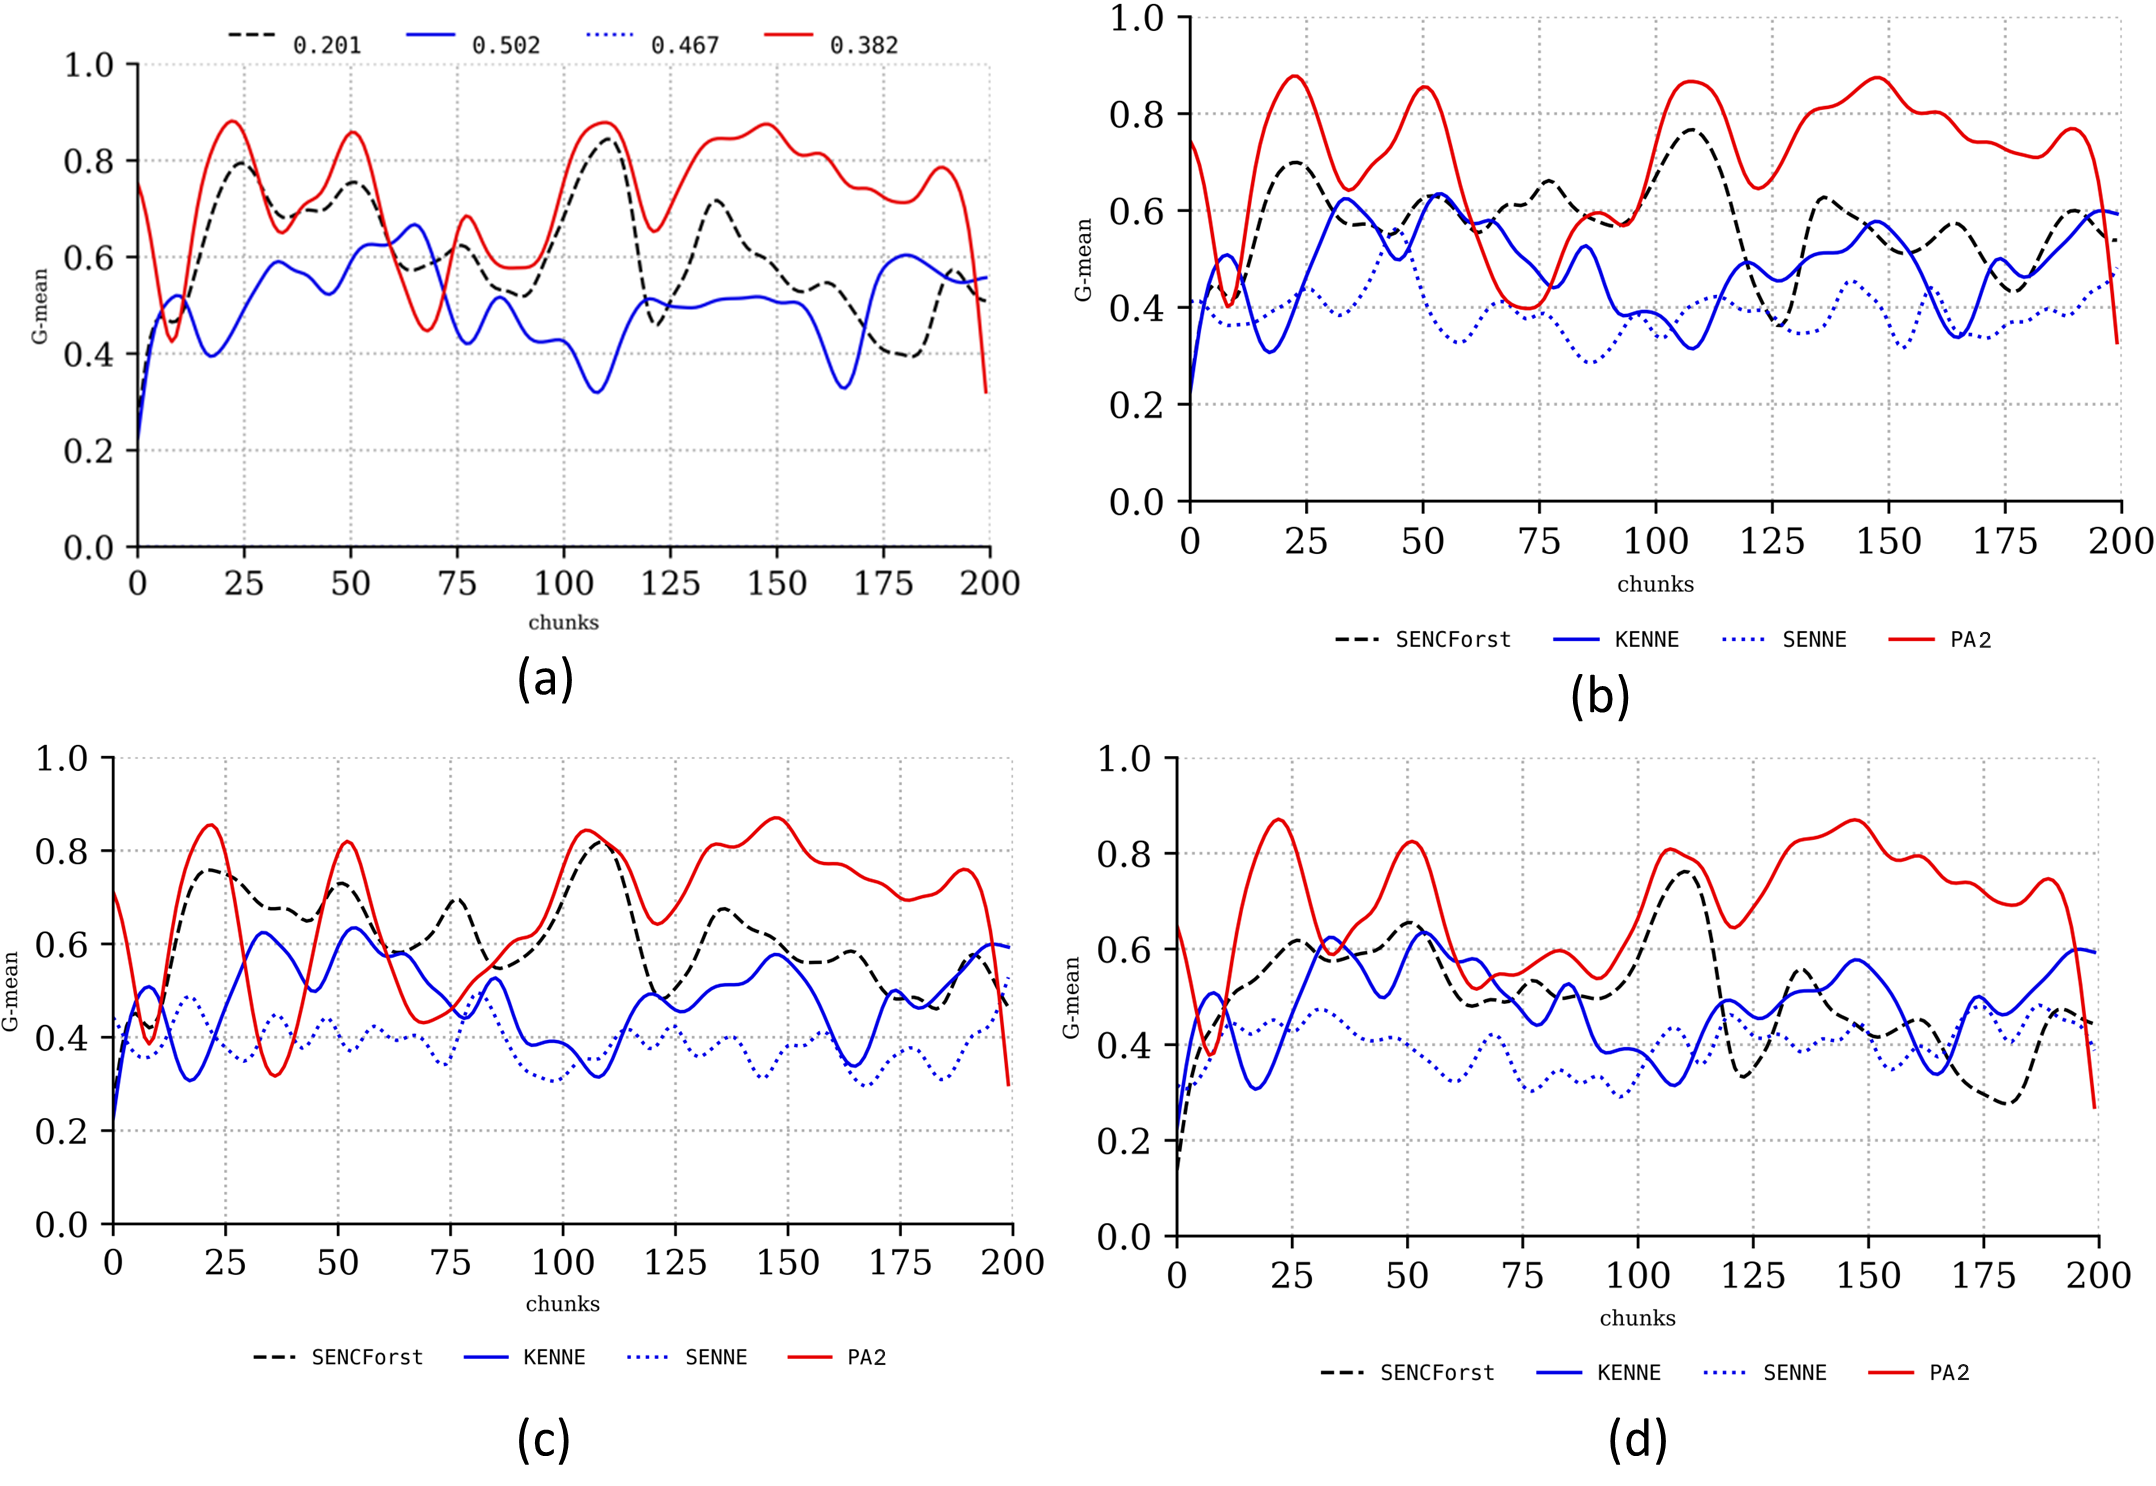
\includegraphics[width=1\linewidth]{5_Emerging/images/res1.png}
	\caption{Covertype stream for various emerging buffer sizes: (a) buffer size of 5, (b) buffer size of 10, (c) buffer size of 20, and (d) adaptive buffer size.}

	\label{fig:res1}
\end{figure}				

\subsubsection{Results On Real Application Stream}
\label{sec:sensor}
This experiment focused on assessing the accuracy of SENCForest, SENNE, KENNES, and PA across 200 chunks of a sensor data stream, utilizing varying buffer sizes similar to the previous experiment. The results, shown in Fig. \ref{fig:res2}, were visualized using scatter plots. Fig. \ref{fig:res2} (a) displays the classification accuracy for each algorithm with a buffer size of 5. The PA algorithm achieved the highest performance overall, except for chunks 43 to 48, where some instances were incorrectly assumed as outliers rather than emergent. In contrast, SENCForest and SENNE had the lowest accuracy. Additional experiments with buffer sizes of 10 and 20 (Fig. \ref{fig:res2}(b) and Fig. \ref{fig:res2}(c)) demonstrated reduced accuracy compared to the buffer size of 5, attributed to fewer updates with larger buffer sizes. The adaptive buffer size experiment in Fig. \ref{fig:res2}(d) reaffirmed the effectiveness of the PA algorithm, which outperformed others across all chunks, with the adaptive emerging pool size providing optimal results.

\begin{figure}[!ht]
	\centering
	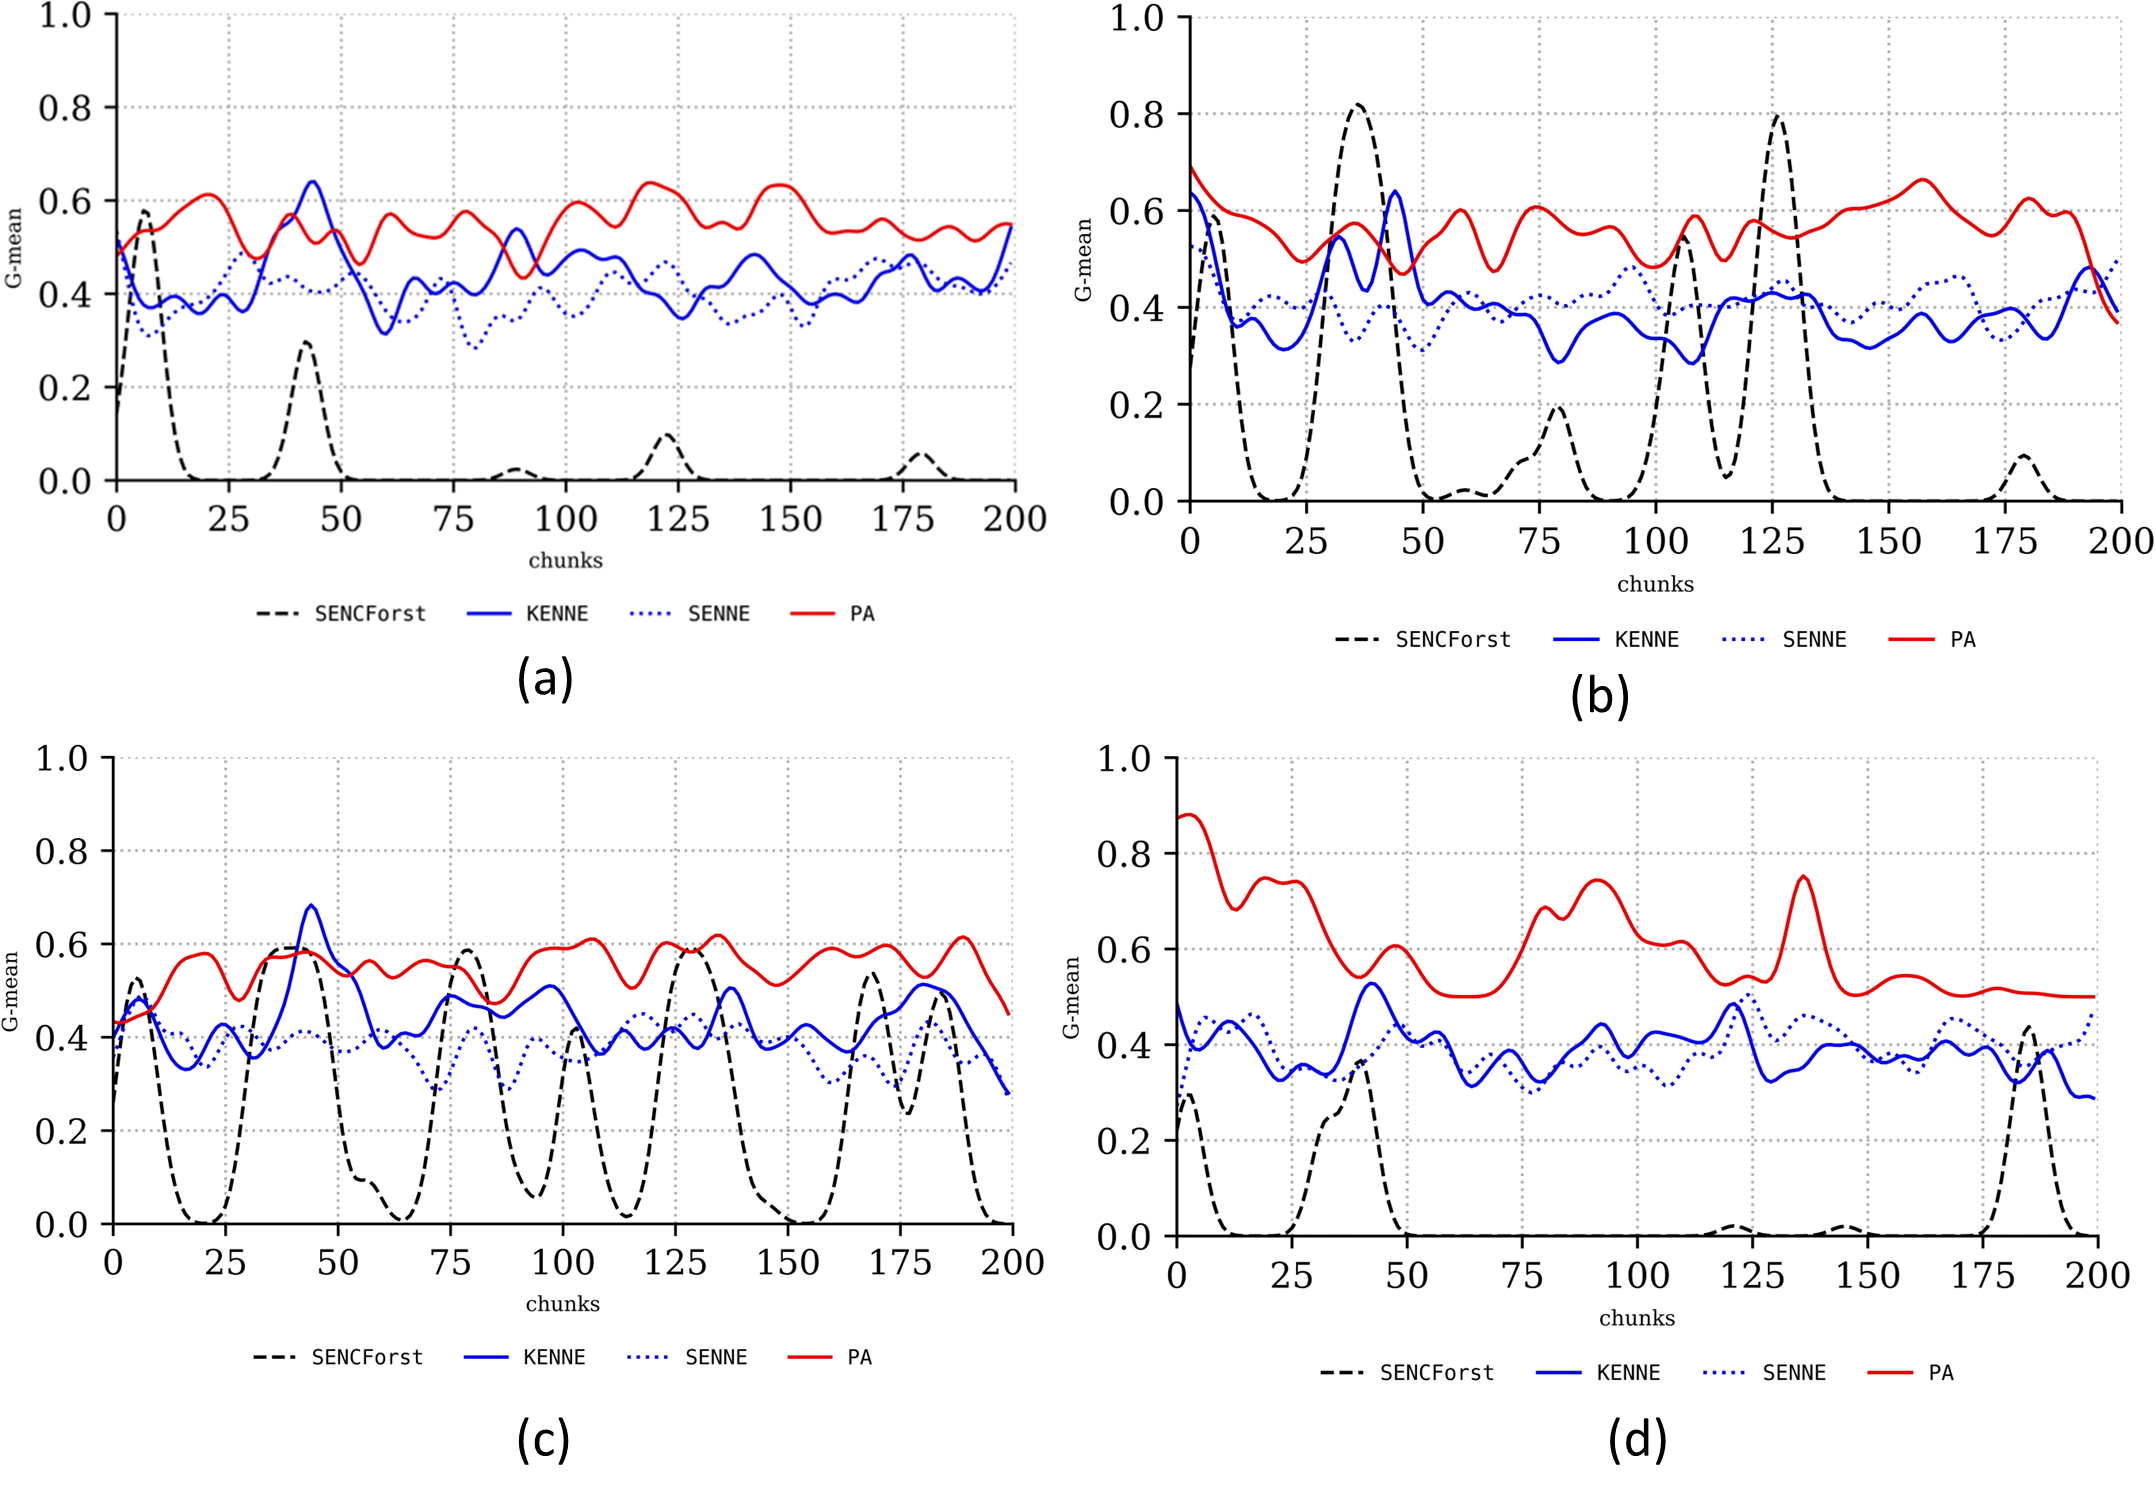
\includegraphics[width=1\linewidth]{5_Emerging/images/res2.png}
	\caption{Sensor stream for various emerging buffer sizes: (a) buffer size of 5, (b) buffer size of 10, (c) buffer size of 20, and (d) adaptive buffer size.}

	\label{fig:res2}
\end{figure}				

\subsubsection{Results On Synthetic Stream}
\label{sec:synthetic}
This experiment aimed to assess the performance of the previously tested methods on a synthetic data stream. Results, depicted in Fig. \ref{fig:res3}, were analyzed using radar and scatter plots. Fig. \ref{fig:res3}(a) shows the performance of various algorithms using a buffer size of 5, with the radar plot highlighting PA's superior performance. Scatter plots illustrate that PA consistently delivered the highest accuracy when applied to the synthetic stream with buffer sizes of 5, 10, and 20, as shown in Fig. \ref{fig:res3}(a), Fig. \ref{fig:res3}(b), and Fig. \ref{fig:res3}(c), respectively. Fig. \ref{fig:res3}(d) demonstrates that the adaptive pool size yielded the best accuracy on the synthetic stream, underscoring the adaptability and efficiency of the PA algorithm.

\begin{figure}[!ht]
	\centering
	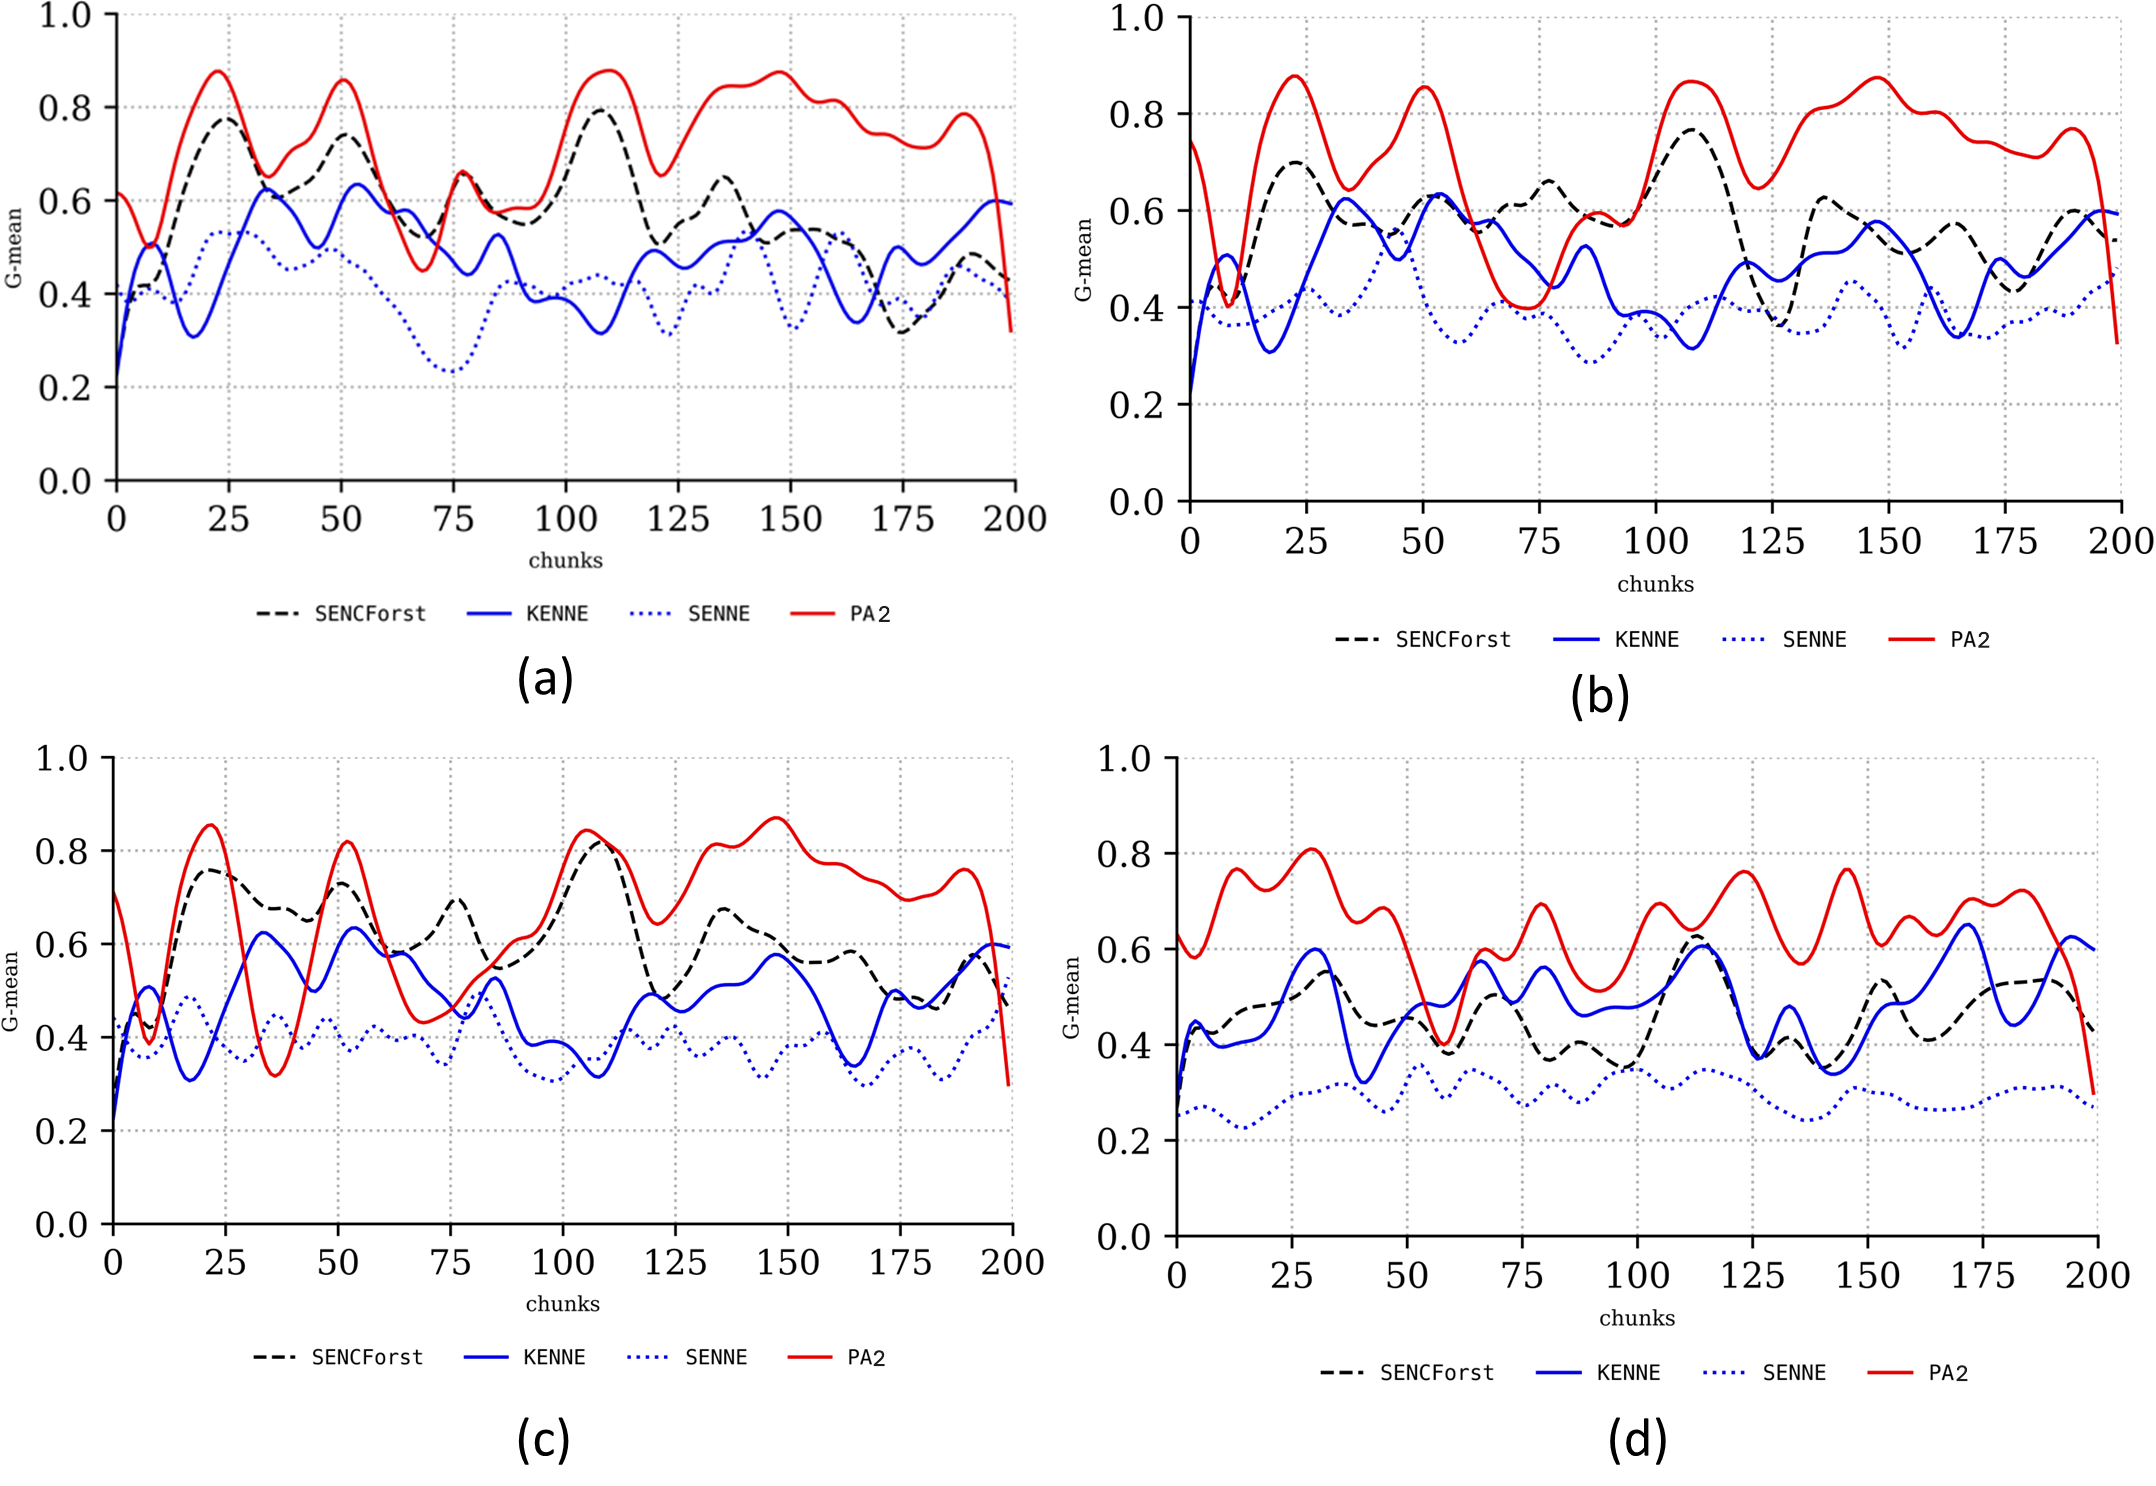
\includegraphics[width=1\linewidth]{5_Emerging/images/res3.png}
	\caption{Synthetic stream for various emerging buffer sizes: (a) buffer size of 5, (b) buffer size of 10, (c) buffer size of 20, and (d) adaptive buffer size.}

	\label{fig:res3}
\end{figure}				

\subsection{Runtime Analysis Of The Best Algorithms}
\label{sec:running}
Our experimental results revealed that selecting the optimal algorithm for detecting emerging new classes is influenced by various factors, including dataset characteristics, buffer length, and the algorithm's runtime requirements. We conducted a series of experiments to evaluate the runtime performance of different algorithms and observed that the PA algorithm demonstrated outstanding efficiency. Specifically, with the adaptive pool size approach, the PA algorithm trained bagging classifiers 150 times within 2131 seconds when using the Covertype stream, outperforming others despite SENCForest achieving the lowest runtime but with fewer updates compared to PA as shown in Table \ref{table:table_2}. On the Sensor stream, PA delivered the best runtime for 66 updates, while SENCForest, KENNES, and SENNE required more time to complete the same or fewer iterations. Similarly, PA exhibited superior runtime performance on the Synthetic stream. These results underscore the PA algorithm’s efficiency, making it an ideal choice for time-constrained scenarios. The superior runtime performance of PA is further highlighted in bold in Table \ref{table:table_2}.
	
\begin{table}[t]
	\centering
	\caption{Running time of SENCForest, SENNE, KENNE, and the Proposed Approach (PA).}
  \resizebox{\textwidth}{!}{
	\begin{tabular}{|l|l|c|c|}
	\hline
	\textbf{Stream}    & \textbf{Algorithm} & \textbf{Training Times} & \textbf{Time (seconds)} \\ \hline
	Covertype          & SENCForest         & 142                     & \textbf{1997}           \\ \cline{2-4} 
					   & SENNE              & 5                       & 2167                    \\ \cline{2-4} 
					   & KENNES             & 3                       & 1742                    \\ \cline{2-4} 
					   & PA                 & 150                     & 2131                    \\ \hline
	Sensor             & SENCForest         & 23                      & 1244                    \\ \cline{2-4} 
					   & SENNE              & 17                      & 3825                    \\ \cline{2-4} 
					   & KENNES             & 152                     & 2109                    \\ \cline{2-4} 
					   & PA                 & 66                      & \textbf{1075}           \\ \hline
	Synthetic          & SENCForest         & 12                      & 107                     \\ \cline{2-4} 
					   & SENNE              & 26                      & 224                     \\ \cline{2-4} 
					   & KENNES             & 149                     & 202                     \\ \cline{2-4} 
					   & PA                 & 47                      & \textbf{91}             \\ \hline
	\end{tabular}
  }

	\label{table:table_2}
	\end{table}

\subsection{Comparison between GNB, KNN, and HT, SVC}
\label{sec:compared_base_calssfier}
In this section, we compare various algorithms (KNN, SVC, GNB, and HT) as base classifiers for the bagging technique. The comparison, illustrated in Fig.\ref{fig:res4}, focuses on the Covertype dataset stream, where GNB (blue line) and HT (red line) consistently achieve the highest scores across most chunks. Both classifiers also excel in radar plots across key performance metrics, including accuracy, precision, recall, and F1-score. Based on these results, GNB and HT emerge as the most suitable base classifiers for the bagging technique. We further compared GNB and HT in terms of runtime and update frequency, as shown in Table \ref{table:table_3}. The results indicate that GNB has the best runtime performance, while HT demonstrates superior accuracy, likely due to its higher number of updates compared to GNB, as reflected in Table \ref{table:table_3} and Fig. \ref{fig:res4}.

\begin{figure}[t]
	\centering
	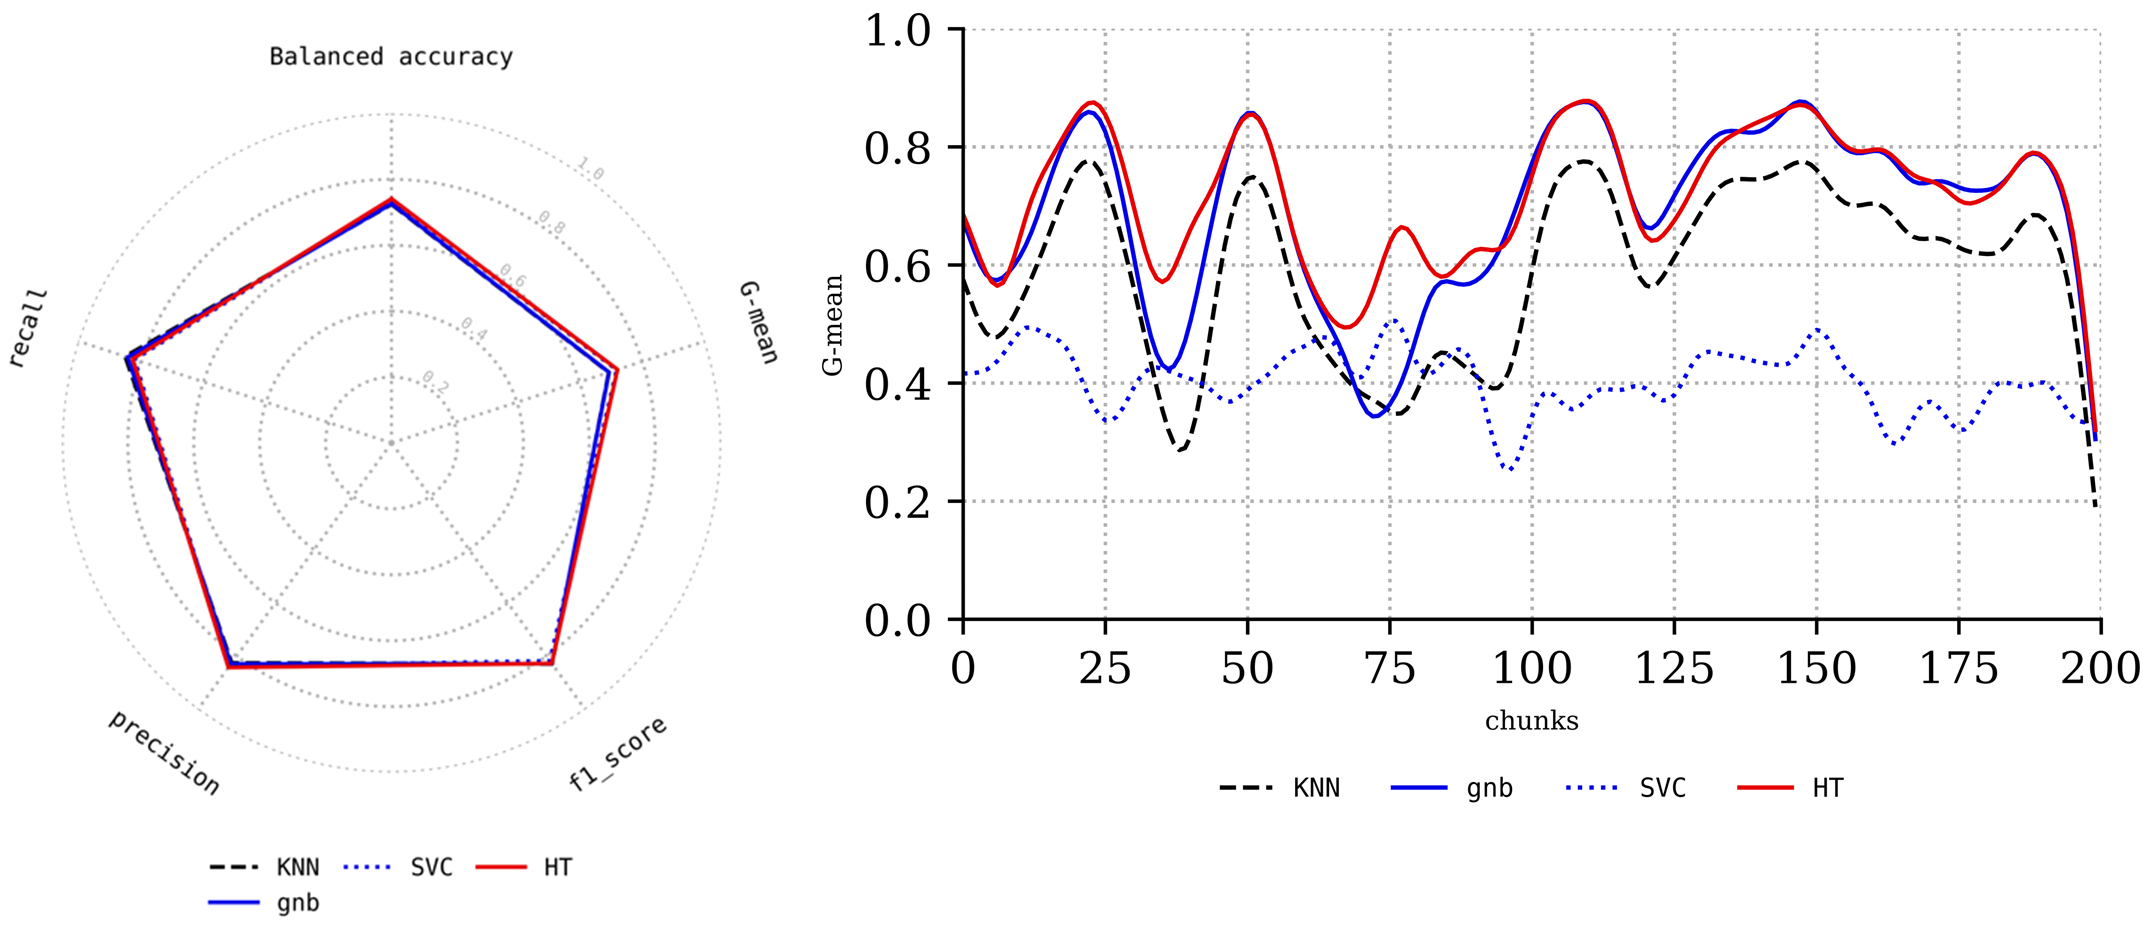
\includegraphics[width=1\linewidth]{5_Emerging/images/res4.png}
	\caption{Covertype stream for concept drift detectors (ADWIN, DDM) evaluated using several metrics: recall, precision, balanced accuracy, G-mean, and F1 score.}

	\label{fig:res4}
\end{figure}				

	
\begin{table}[t]
	\centering
	\caption{Running time of KNN, SVC, GNB, and HT as base classifiers.}
	\begin{tabular}{|l|c|c|c|c|}
	\hline
	\textbf{Algorithm}     & \textbf{KNN} & \textbf{SVC} & \textbf{GNB} & \textbf{HT} \\ \hline
		Training Times         & 140          & 150          & \textbf{139} & 148         \\ \hline
		Time (seconds)         & 586          & 878          & \textbf{291} & 1169        \\ \hline
	\end{tabular}
	\label{table:table_3}
	\end{table}


\subsection{Comparison between ADWIN and DDM}
\label{sec:compared_drift_detector}
In this section, we compare two concept drift detection methods: the Drift Detection Method (DDM) \cite{gama2004learning} and the Adaptive Window (ADWIN) \cite{gama2004learning, adams2023explainable}. These methods are widely recognized for their excellent performance in handling incremental drifted streams \cite{gama2004learning, adams2023explainable, madkour2023historical, baena2006early}. As shown in Fig. \ref{fig:res5}, using the Synthetic stream with GNB as the base classifier, ADWIN consistently outperforms DDM in both radar and line plots across all performance metrics, including accuracy. Furthermore, when comparing their runtime and update frequency, as presented in Table \ref{table:table_4}, ADWIN proves to be the superior detector for drifted streams. It identifies the highest number of drifts (139) in the least amount of time (272 seconds), demonstrating its efficiency and effectiveness.
\begin{figure}[!ht]
	\centering
	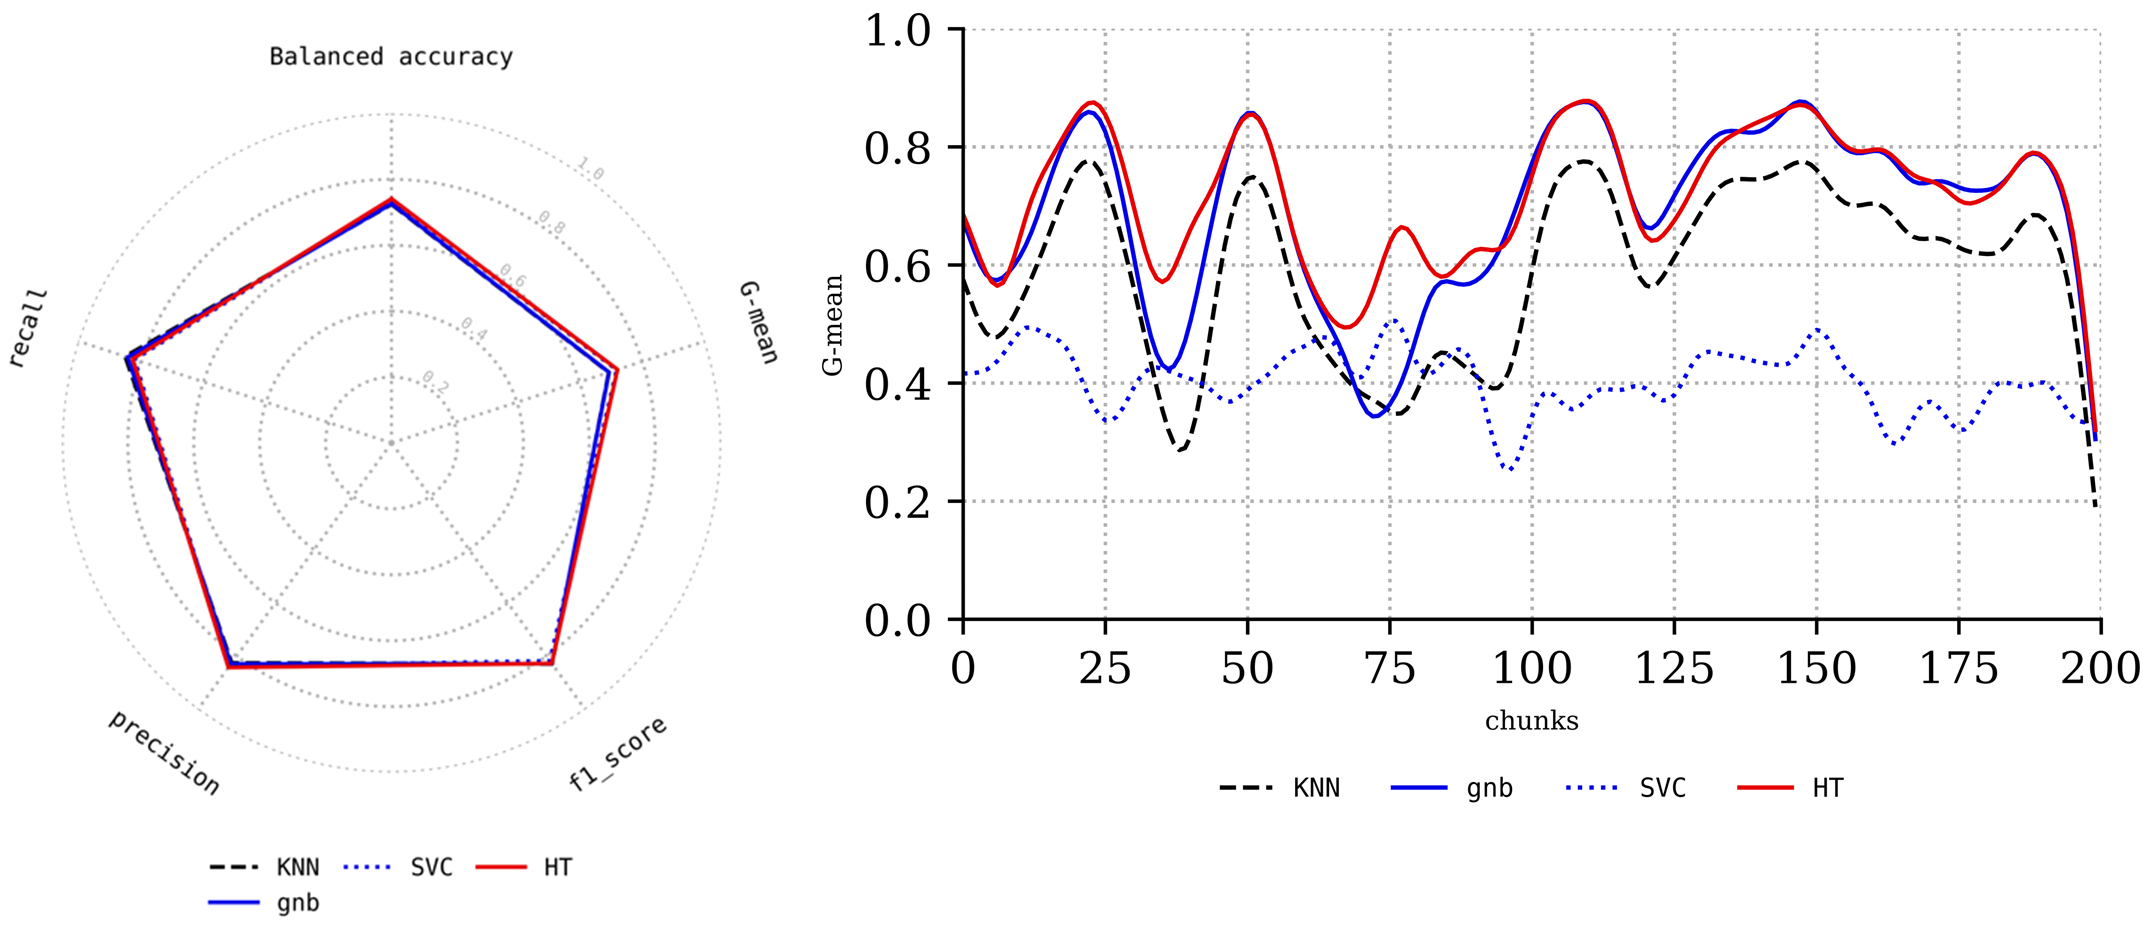
\includegraphics[width=1\linewidth]{5_Emerging/images/res4.png}
	\caption{Synthetic stream for concept drift detectors (ADWIN, DDM) evaluated using several metrics: recall, precision, balanced accuracy, mean, and F1 score.}

	\label{fig:res5}
\end{figure}
	
\begin{table}[!ht]
	\centering
	\caption{Running time of ADWIN and DDM as drift detectors.}
	\begin{tabular}{|l|c|c|}
		\hline
	\textbf{Algorithm}     & \textbf{ADWIN} & \textbf{DDM}  \\ \hline
Training Times         & 139          & 55                   \\ \hline
Time (seconds)         & 272          & 545                   \\ \hline
	
	\end{tabular}
	\label{table:table_4}
	\end{table}